% ============================================================================
%  RTAS 2027 submission — new paper (started 2026-10-23)
%
%  Paper/ : the frozen 2026-09-28 negative-result draft. It is SOURCE MATERIAL
%           only (LaTeX shell, refs, background measurements). Do not submit it.
%
%  写作纪律（本项目的硬规矩，改正文时守住）：
%   1. 每一个数字要么来自 scripts/lab/*.py 的产物（paper2027/data/*.csv），
%      要么标 \pend{}。不许手抄，不许估。
%   2. \pend{...} = 数字未落地。正文里出现 \pend 的地方，PENDING.md 必须有对应条目。
%      投稿前 `grep -c '\pend{'` 必须是 0。
%   3. 不写"显著"、不写置信区间、不写 3--4x（n=1）。
%   4. 不宣称 agent-level admission（CONCUR）、per-tier admission（MORI）、
%      working-set admission（EfficientAgent）。
%   5. 只投这一篇。
% ============================================================================
\documentclass[10pt,conference]{IEEEtran}
\usepackage{cite}
\usepackage{amsmath,amssymb}
\usepackage{graphicx}
\usepackage{booktabs}
\usepackage{url}
\usepackage[hidelinks]{hyperref}
\usepackage{xcolor}
\usepackage{caption}

% ---- 未落地的数字：红色、方括号、可 grep -------------------------------
\newcommand{\pend}[1]{\textcolor{red}{[PENDING: #1]}}
% ---- 系统名 -----------------------------------------------------------
\newcommand{\sys}{\textsc{Foyer}}
% ---- 常用符号 ---------------------------------------------------------
\newcommand{\Wset}{W}
\newcommand{\Ceff}{C_{\mathrm{eff}}}
\newcommand{\Trev}{T_{\mathrm{rev}}}
\newcommand{\Trec}{T_{\mathrm{rec}}}

\begin{document}

\title{Admission Is a Feasibility Test, Not a Threshold:\\
Capacity Accounting and Revival Pricing for Agentic LLM Serving}

% RTAS 2027 是双盲（double-anonymous）。作者栏在投稿版必须保持匿名。
\author{\IEEEauthorblockN{Anonymous Submission}}

\maketitle

\begin{abstract}
An agentic LLM session is a long, multi-round job. Every round returns with a context
that has grown, so a session's KV footprint is large, durable, and reused---and on a
single GPU the live working set can exceed the KV pool by an order of magnitude.
Existing systems frame this as placement, and placement forces prediction: which prefix
will be reused, when a session will come back, how long the next round will be. We argue
the prediction is unnecessary. A session can be \emph{suspended} at a round boundary and
\emph{revived} by copying its KV back---when the host tier still holds it---instead of
recomputing it; admission then becomes a
feasibility test over a capacity ledger---does this session's projected footprint fit,
now, on which tier, and at what revival cost. We give a feasible-set bound, a
session-level revival-versus-recompute break-even, and a coverage-bounded growth estimate
that turns the safety margin into a stated property rather than a constant. On a
19-session, 602-round coding-agent replay, the terminal working set is 12.9$\times$ the
KV pool and a mean session needs 69K of its 101K tokens, so the pool holds
1.47 mean sessions. Replaying every round as an independent request re-reads
13$\times$ more prefix than it appends. We instantiate the design on SGLang with a
two-tier KV cache and compare it against request-level serving and an agent-level
feedback controller: \pend{headline number}. We also state where the mechanism loses---
when the working set fits, and when revival costs as much as recomputation.
\end{abstract}

\begin{IEEEkeywords}
LLM serving, agentic workloads, KV cache, admission control, capacity accounting,
performance evaluation
\end{IEEEkeywords}

\section{Introduction}
\label{sec:intro}

A coding agent does not issue one request. It issues a \emph{session}: a multi-round job
in which every round ends with a tool call, and every tool call returns with more context
than the round before. The session is long-lived, its state is expensive to rebuild, and
it is reused. On a serving engine that was designed for independent requests, none of
these three properties is visible.

We measured this on a replay of 19 long coding-agent sessions (602 rounds, median 28
rounds per session, longest 81) collected from Claude and Codex conversations. A round
arrives with a median 48.5K-token context (p90 71.1K, max 92.8K). The terminal working
set---what all 19 sessions would occupy if every one of them were live---is 1.31M tokens.
The KV pool of our engine, a 7B model served with a 96K context on a single 24\,GB GPU,
holds 101.5K tokens. The working set is therefore $12.9\times$ the pool, and the average
session alone needs 69K tokens: \emph{the pool holds 1.47 sessions}.

The cost of ignoring this is paid every round. A round's new content is a median of 990
tokens, but it arrives attached to a 44.9K-token prefix. Serving each round as an
independent request re-reads that prefix: across the trace, the engine is asked to
process $13.0\times$ more prefix than it appends, and a system with no reuse at all would
do $14.0\times$ the prefill work of a perfect one. The trace makes the same point in the
other direction: it is cheap to keep a session, and expensive to rebuild it.

The obvious response---evict and recompute---runs into the shape of the workload rather
than its size. Tool waits are bimodal: the median gap between rounds is 181\,ms, the mean
is 15.9\,s, and the 13.1\% of gaps longer than ten seconds account for 93.4\% of all
parked time. A session's idle period therefore tells you almost nothing about the next
one: half of the time the agent is back before an eviction decision could pay for itself,
and the other half it is gone for tens of seconds. A policy that suspends on every gap
recomputes constantly; a policy that never suspends holds sessions it cannot afford.

\paragraph{Prior fixes treat this as placement, and placement forces prediction}
Paged attention, prefix caching, and tiered KV stores decide \emph{where} a block lives;
their admission counterpart is a replacement decision that presupposes a guess about the
future---which prefix will be reused, when a session will return, how long its next round
will be. The systems that address agentic workloads keep that presupposition: TTL-based
scheduling predicts a session's reuse window, program-aware admission predicts the next
step's demand, feedback controllers adjust a concurrency limit after congestion is
observed, and overload handlers shed sessions outright. Each is a threshold on a
predicted quantity. None of them states which set of sessions is \emph{feasible} under
the capacity it actually has, and none prices what it costs to bring a suspended session
back.

\paragraph{Our position: make the session suspendable, then stop predicting}
If a session can be paused at a round boundary and resumed by \emph{copying} its KV back
from a host tier, then the question ``should this session be admitted?'' stops being a
forecast and becomes an accounting check against a ledger of bytes:
\begin{quote}
\emph{Admission is a feasibility test, not a threshold.}
\end{quote}
Three things follow, and they organise the paper. First, feasibility is stated in
quantities we can measure now---the session's projected footprint, the capacity of each
tier, the bandwidth between them---so no predictor is on the critical path. Second,
suspension is not free and not always right: reviving a session costs a copy, recomputing
it costs a prefill, and the two are comparable for short contexts, which yields a
per-session break-even instead of a policy constant. Third, the one genuinely uncertain
quantity, how much a session will grow before it returns, is small enough---a few percent
of the footprint it protects---that a crude estimate of it cannot move the ledger, which is
why the design needs no predictor.

\paragraph{Contributions}
\begin{enumerate}
\item \textbf{Formulation} (\S\ref{sec:model}): we cast admission for suspendable agent
sessions as a feasibility problem over a two-tier capacity ledger, with an explicit
revival cost. The formulation replaces a threshold on predicted load with a test on
measured capacity, and it exposes the one parameter that remains---the fraction of the
pool held in reserve (\S\ref{sec:design}).
\item \textbf{Mechanism} (\S\ref{sec:design}--\ref{sec:impl}): named permits make the
ledger enforceable at request granularity; reversible suspension at round boundaries
keeps a session's state in the host tier instead of discarding it; a growth reserve
estimated from the session's own history replaces a point forecast; and the admission
accounting is dominated by measured bytes rather than by that estimate. We implement the design on SGLang with a
hierarchical KV cache and a 96K-context 7B model.
\item \textbf{Analysis and evidence} (\S\ref{sec:analysis}, \S\ref{sec:eval}): we give a
feasible-set bound, a session-level revival-versus-recompute break-even, and a bound on
the projection error; we evaluate request-level serving, an agent-level
feedback controller, and our design on the same trace, engine, and memory budget; and we
report the regimes in which suspension does not pay.
\end{enumerate}

\paragraph{Results in one line}
\pend{one-sentence headline with the three arms, e.g.\ ``on the 602-round replay our
design finishes the batch in X minutes against Y (request-level) and Z (agent-level),
while meeting the per-round deadline on W\% of rounds against V\% and U\%''}.

\paragraph{Scope}
Our testbed is a single 24\,GB GPU running a 7B model with a 96K context. We choose this
point because it makes the regime sharp, not because the mechanism is specific to the
card: the binding variable is the ratio of the live working set to KV capacity, and when
that ratio is small, admission is not the problem. We do not claim that our constants
transfer to larger devices or to clusters; we do claim that the ledger, the break-even,
and the projection bound are stated in quantities---bytes, bandwidth, session
horizon---that do transfer (\S\ref{sec:discussion}).

\section{Background: What a Long Session Costs}
\label{sec:background}

\subsection{The replay}

Our workload is a replay of 19 coding-agent sessions (602 rounds) reconstructed from real
Claude and Codex transcripts released with a public coding-agent characterization study
\cite{zhu2026tracelab}. We keep every session with at least 20 rounds and sample by a hash
of the session identifier, which yields the 19 longest sessions rather than a
hand-picked subset; the trace and the script that rebuilds it are in the artifact. Each
round carries the prefix it can reuse, the new tokens it appends, the number of tokens the
model is asked to emit, an inter-round tool wait, and an arrival time. All sessions arrive
at $t=0$: we model the batch-of-agents case (a nightly evaluation, a benchmark sweep, a
fleet of assistants started together), which is the case that stresses admission hardest
and the case an offline batch server is actually configured for.

\begin{figure}[t]
\centering
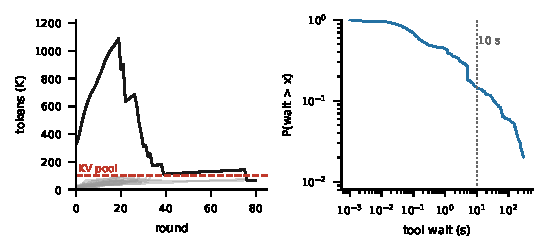
\includegraphics[width=\columnwidth]{figs/fig_workload.pdf}
\caption{Left: the working set if every session alive at that round were resident (black),
against the engine's KV pool (dashed). The aggregate peaks above one million tokens---ten
times the pool---while no single session's context ever exceeds the pool on its own.
Summing every session's terminal context gives 1.31M tokens, $12.9\times$ the pool. Right:
the tool wait between rounds, as a complementary CDF. The distribution is bimodal: half of
the gaps are under 0.2\,s, and the 13.1\% above ten seconds carry 93.4\% of the parked
time.}
\label{fig:workload}
\end{figure}

\subsection{Four numbers that decide the design}

Table~\ref{tab:workload} collects the characterisation and Fig.~\ref{fig:workload}
shows its two shapes; every entry is regenerated from the trace by
\texttt{gen\_trace\_facts.py}. Four of them drive everything that follows.

\paragraph{The working set is an order of magnitude larger than the pool}
The terminal footprint of all 19 sessions is 1.31M tokens. The engine's KV pool on a
24\,GB card with a 96K context and a 7B model is 101.5K tokens. The ratio is
$12.9\times$, and a mean session (69K tokens) already needs two thirds of the pool: the
pool holds 1.47 sessions. There is no scheduling policy that makes 19 sessions resident;
the question is only which subset is resident at each instant.

\paragraph{Almost all of the work is re-reading}
A round appends a median of 990 tokens to a median 44.9K-token prefix. Aggregated over the
trace, the prefix is $13.0\times$ the appended content, and the prefill work of a system
with no reuse would be $14.0\times$ that of a system that never re-reads a prefix. This
gap is the prize: the engine spends its time on prefill of content it has already seen.

\paragraph{Reuse is worth a lot, and it is perishable}
Because a session's context only grows, the prefix of round $i$ is a prefix of round
$i+1$: a single retained copy serves every later round. But retention competes with
admission---every token held for a parked session is a token an active session cannot
use---so reuse and capacity are two views of the same decision, not two separate
optimisations.

\paragraph{Idle time is bimodal, so ``park'' is not one thing}
The median gap between rounds is 181\,ms; the mean is 15.9\,s; the 90th percentile is
28.1\,s and the maximum is the trace's 300\,s timeout. The 13.1\% of gaps above ten
seconds carry 93.4\% of all parked time: across the trace the sessions sit idle for 2.65
hours in total, and 2.47 of those hours are in long gaps. A gap of 181\,ms is shorter than
the cost of moving a 44.9K-token prefix anywhere, while a gap of 28\,s is longer than the
prefill that would rebuild it. Any single policy---always keep, always evict---is wrong
for at least half of the gaps.

\begin{table}[t]
\caption{Workload characterisation of the 19-session, 602-round replay. Context is
measured at the start of a round; the working set sums the terminal context of each
session. All values are recomputed from the trace by \texttt{gen\_trace\_facts.py}.}
\label{tab:workload}
\centering
\small
\begin{tabular}{@{}lr@{}}
\toprule
Quantity & Value \\
\midrule
sessions / rounds & 19 / 602 \\
rounds per session (median / max) & 28 / 81 \\
context per round (median / mean) & 48.5K / 48.2K \\
context per round (p90 / max) & 71.1K / 92.8K \\
terminal working set & 1.31M tokens \\
KV pool (device tier) & 101.5K tokens \\
working set / pool & $12.9\times$ \\
mean session footprint & 69.0K tokens \\
pool in mean sessions & 1.47 \\
appended tokens per round (median) & 990 \\
reusable prefix per round (median) & 44.9K \\
prefix / append, per round (median) & $45.4\times$ \\
prefix / append, whole trace & $13.0\times$ \\
recompute / append bound & $14.0\times$ \\
tool wait p50 / mean & 181\,ms / 15.9\,s \\
tool wait p90 / max & 28.1\,s / 300\,s \\
gaps $>10$\,s (share of gaps / of time) & 13.1\% / 93.4\% \\
\bottomrule
\end{tabular}
\end{table}

\subsection{What a round does to the engine}

A round is a prefill of the full context followed by a short decode: 48.5K tokens in,
about 150 tokens out. On the 24\,GB card the prefill of a cold 44.9K-token prefix takes
about 100\,s (median 103\,s over the 131 cold rounds of one run) and the decode is a fraction of a second; when the
prefix is resident, the same round costs a few milliseconds of copy and a prefill of the
990 new tokens. The engine therefore has two very different operating points, and the
whole question of this paper is how often it can be in the second one.

\subsection{The engine and its memory hierarchy}

We use SGLang \cite{zheng2024sglang} with paged KV \cite{kwon2023pagedattention} and its
hierarchical cache, which extends the device pool with a host pool at a configurable ratio
(we use $2\times$, i.e.\ 203K tokens in host memory). The hierarchy is the substrate that
makes suspension meaningful: the host tier is where a suspended session can wait without
occupying the card, and the PCIe link is the price of putting it back. The engine itself
does not have a notion of a session, so it cannot tell a cache miss caused by a new
session from one caused by an evicted session that is about to return. Supplying that
notion is the job of the design in \S\ref{sec:design}.

\section{Model}
\label{sec:model}

\subsection{Sessions, rounds, and state}

A \emph{session} $s$ is a sequence of rounds $i=1,\dots,n_s$, arriving at time $a_s$.
Round $i$ carries a reusable prefix of $p_{s,i}$ tokens, appends $q_{s,i}$ tokens, and
asks for $o_{s,i}$ output tokens, so the context served by the engine is
$c_{s,i}=p_{s,i}+q_{s,i}$ and the KV state after the round occupies
$\Phi_{s,i}=\kappa\,(c_{s,i}+o_{s,i})$ bytes for $\kappa$ bytes per token. Between rounds
the session is idle for $w_{s,i}$ (the tool call), which in our trace is drawn from a
bimodal distribution (\S\ref{sec:background}). Because a session only appends, the prefix
of round $i$ is a prefix of every later round: the reuse unit is the session, not the
request.

At any instant a live session is in one of three \emph{states}: \emph{resident} (its KV is
in the device pool, so its next round prefills only $q_{s,i}$), \emph{suspended} (its KV
is in the host tier, so its next round costs a copy plus $q_{s,i}$), or \emph{absent} (its
state is gone, so its next round prefills all of $c_{s,i}$). The engine we build on
implements the first and third; the design in \S\ref{sec:design} adds the second.

\subsection{Capacity and the feasible set}

Let the device tier hold $C_d$ tokens and the host tier $C_h$ tokens, and let $\rho\in(0,1]$
be the fraction of the device pool the admission policy is allowed to commit. At time $t$
let $A(t)$ be the resident set and $H(t)$ the suspended set. Feasibility is
\begin{equation}
\sum_{s\in A(t)}\Phi_s(t)\;\le\;\rho\,C_d,
\qquad
\sum_{s\in H(t)}\Phi_s(t)\;\le\;C_h .
\label{eq:feasible}
\end{equation}
The \emph{feasible set} $\mathcal{F}(t)$ is the collection of resident sets satisfying
\eqref{eq:feasible}; admission is the choice of $A(t)$, not of a concurrency count. This is
the formal content of our claim. A threshold policy fixes $|A(t)|\le k$; because
$\Phi_s$ varies by $2\times$ across sessions and by $2\times$ within a session over its
life, a fixed $k$ is either infeasible for some $t$ or leaves capacity unused at others.
The bound in \S\ref{sec:analysis} makes the gap explicit.

\subsection{Two costs: revive or recompute}

Bringing a session back has two possible prices. Copying it back from the host tier costs
\begin{equation}
\Trev(s)\;=\;\frac{\Phi_s}{B}\;+\;\tau ,
\label{eq:trev}
\end{equation}
where $B$ is the effective host-to-device bandwidth and $\tau$ the fixed cost of
restoring a sequence in the engine (allocation, descriptor rebuild, first-token
latency). Recomputing the round from scratch costs the prefill of the whole context,
\begin{equation}
\Trec(s)\;=\;P\!\left(c_{s}\right),
\label{eq:trec}
\end{equation}
with $P$ the prefill latency of the engine at the current batch load. For our workload
the two are within a factor of a few: a 45K-token prefill on the 24\,GB card takes
about 100\,s, while copying the corresponding 2.5\,GB of KV at \pend{GB/s}
takes \pend{copy time}. Neither dominates, which is why the decision has to be priced
rather than hard-coded.

\subsection{Assumptions}

We state the assumptions that the analysis uses, so that the guarantees are not read more
broadly than they hold.
\begin{enumerate}
\item \textbf{Round-boundary suspension.} A session is suspended only between rounds. A
round in flight is never preempted; this matches the engine, whose KV for an active
sequence cannot be moved mid-decode.
\item \textbf{Monotone growth.} Within a session the context grows: $c_{s,i+1}\ge c_{s,i}$.
This holds in our trace and in the agent workloads we are aware of, and it is what makes
a retained prefix reusable.
\item \textbf{Known per-token cost.} $\kappa$, $B$, and $\tau$ are measured once on the
deployment and are stable across sessions. We do not model bandwidth contention between
concurrent copies.
\item \textbf{Host capacity is finite and shared.} $C_h$ is a real budget; suspending
always has a victim when the host is full. This is what makes the break-even a
\emph{replacement} condition rather than a per-session one.
\item \textbf{Growth is estimated from observed history, not modelled.} The reserve
$\hat g_s$ is a statistic of the session's own completed rounds (\S\ref{sec:m3}); the
analysis bounds how far its error can move the projection.
\end{enumerate}

\section{Design}
\label{sec:design}

The design has one idea and four mechanisms. The idea is that the controller should keep
a byte-accurate account of which session occupies which tier, and should make every
admission decision against that account. The mechanisms are what it takes to keep the
account true: a way to \emph{enforce} it (\S\ref{sec:m1}), a way to \emph{hold} a session
that is not being served (\S\ref{sec:m2}), a way to \emph{reserve} room for growth
(\S\ref{sec:m3}), and a way to \emph{price} the two decisions the account cannot make by
itself (\S\ref{sec:m4}). Figure~\ref{fig:overview} shows the control path.

\subsection{M1: a capacity ledger with named permits}
\label{sec:m1}

The controller keeps one entry per live session,
$\ell_s=(\text{id},\text{tier},\hat\Phi_s)$, where $\hat\Phi_s$ is the projected footprint
the session needs for its next round. The projection has two parts: the session's
\emph{measured} resident context---the prompt length of its completed rounds, as reported
by the engine---and a growth reserve $\hat g_s$ (\S\ref{sec:m3}). The ledger maintains
$\sum_{s\in A}\hat\Phi_s$ and $\sum_{s\in H}\hat\Phi_s$ and checks them against
\eqref{eq:feasible} before every decision.

Accounting alone is only a model, so the decision is made binding by a \emph{named
permit}. Once per control cycle the controller writes the complete set of session ids
allowed to hold an engine slot, together with the set that is paused; the runner blocks
any session whose id is not in the admit set at its next round boundary. There is no
scalar concurrency limit anywhere in the path: the permit names sessions, so the set the
ledger has accounted for and the set the engine may serve are the same set by
construction. This is what separates the design from a threshold controller---a threshold
changes how many requests may run and hopes the resulting set fits, whereas a permit
cannot be issued until the set has been shown to fit.

\subsection{M2: suspension at round boundaries, not eviction mid-flight}
\label{sec:m2}

When a session is not allowed to continue, the design does not let the engine evict it
mid-round and does not drop its state. The session is \emph{suspended}: it keeps its
ledger entry, its permit identity, and its KV, and it blocks at the next round boundary
until the ledger admits it again. Suspension is a state of the session, not a side effect
of cache replacement.

Two properties make this work in practice. The engine's hierarchical cache keeps the
prefix of an evicted sequence in the host tier, so a suspended session that is admitted
again usually resumes by \emph{copying} its prefix back rather than recomputing it
(\S\ref{sec:analysis} shows the copy is two orders of magnitude cheaper than the
prefill). And the host tier is finite, so suspension is a replacement decision like any
other: admitting a session's state into the host tier means some other session's state
cannot be there. The ledger therefore tracks host occupancy as a first-class sum, and
\S\ref{sec:m4} decides who gets a host slot.

\subsection{M3: reserve for growth from observed growth}
\label{sec:m3}

A session that is admitted now will keep growing while it is resident, so the ledger must
reserve room for the next round. We reserve the session's own recent growth:
\[
\hat g_s=\underbrace{\mathrm{EMA}\bigl(q_{s,j}+o_{s,j}\bigr)}_{\text{own history}}\;\cdot\;h
\]
over the session's completed rounds, where $h$ is the number of rounds the session may run
before the next control decision (three in our runs, with a 1.15 safety factor). For a
session with fewer than three observed rounds the estimate is blended toward a global prior
estimated from all sessions, so a young session is not over-reserved.

The justification for estimating growth so crudely is in the numbers. On the trace the
reserve has a median of 4.0K tokens against a 48.5K-token context---8.2\% of the footprint
it protects---and the ledger charges $1.15\times(\text{context}+\hat g)$, which at the
median is 22.1\% more than the context itself. That margin is not free: it holds back about
10.7K tokens, a tenth of the pool, and it is the price of never under-reserving. The
coverage it buys is complete on this trace: in all 583 round transitions the projection
exceeded the realised next-round footprint (\S\ref{sec:analysis}). A cheaper corner exists
---$h=1$, margin $1.05$ covers 94.5\% of the transitions with 5.3\% slack---but the two
constants were fixed before the evaluation and left alone, and we report the sweep rather
than claiming the deployed corner is optimal.

The measured part of the projection---the resident context, read from the engine's own
records---is what admission actually turns on; the estimated part is under a tenth of it.

\subsection{M4: pricing the two decisions the ledger cannot make}
\label{sec:m4}

The ledger says what fits; it does not say what is worth doing. Two decisions remain, and
both are priced in the same currency---time.

\paragraph{Who gives way, and when} The valve opens when the engine's own utilisation
crosses a hard stop or when the observed first-token latency crosses the round deadline;
the second signal is gated on pressure, so that a long prefill on an otherwise idle card
is not mistaken for congestion. When the valve opens, the controller suspends sessions
until the survivors fit in $0.90$ of the committed budget, and it takes the
\emph{youngest} sessions first: they have the least invested context, so the recompute
they may incur is the smallest, and they are the least likely to have accumulated state
worth keeping. This is the observable form of the per-byte ranking in \S\ref{sec:analysis}:
youngest-first is smallest-$\Trec$ first.

\paragraph{Resuming} A suspended session re-enters the ordinary admission path and is
admitted when the ledger's projection fits. Because its prefix is usually still in the
host tier, resumption is a copy; when the host tier has lost the prefix the same round is
served as a cold prefill, and the accounting charges it as such.

\paragraph{Two refinements, implemented but not enabled} The controller also supports an
idle-time gate on suspension (suspend only after a session has been parked longer than the
time to serve a replacement round, \S\ref{sec:analysis}) and a gate on the number of
\emph{running} sessions rather than live ones. Both were left at their defaults in the runs
we report, so the evaluation measures the ledger, the growth reserve, and youngest-first
shedding alone; we say so because the mechanisms are easy to confuse with the ones that
produced the numbers.

\subsection{The knob}

One parameter remains: the fraction $\rho$ of the pool the ledger is allowed to commit
($\rho=0.95$ in our runs, with the fixpoint pushed to $0.90$ of the budget before shedding).
It is the only tuned quantity in the design. Everything else---the projected footprint,
the resident context, the running count, the observed latency---is measured. We report the
sensitivity of the evaluation to $\rho$ rather than presenting it as a constant of the
mechanism.

\begin{figure}[t]
\centering
\fbox{\parbox{0.92\columnwidth}{\centering\vspace{2.0em}
\textbf{Figure placeholder: control path}\\[0.4em]
\footnotesize
runner $\to$ arrival/pause/resume events $\to$ ledger (resident + $\hat g_s$)\\
$\to$ named permit (admit set, paused set) $\to$ runner gate $\to$ engine\\
engine \texttt{/metrics} $\to$ valve $\to$ shedding (youngest, idle $>t^\ast$)
\vspace{2.0em}}}
\caption{Control path. The permit names sessions, not a count; suspension and resumption
are ledger transitions enforced at round boundaries.}
\label{fig:overview}
\end{figure}

\subsection{What is deliberately absent}

There is no predictor of the next round's length, no estimate of a session's remaining
horizon, and no per-request latency model. The only estimated quantity is a per-session
growth reserve whose error cannot move the ledger by more than a few percent, and the only
tuned quantity is $\rho$. The design degrades gracefully at both ends: with ample capacity
nothing is suspended and the ledger admits first-come-first-served; with short contexts
the growth reserve is negligible and admission is a pure capacity check.

\section{Analysis}
\label{sec:analysis}

We state three results. The first bounds the resident set in sessions and shows why a
concurrency threshold cannot be the right control variable. The second prices a revival
and locates the real scarcity. The third bounds how much a wrong growth reserve can move
the ledger, which is the formal reason the design can afford a crude estimate.

\subsection{Prop.~1: the feasible set is small, and a threshold cannot track it}

Let the live sessions' footprints be $\Phi_{(1)}\le\cdots\le\Phi_{(m)}$ in ascending order
and let $\rho C_d$ be the committed device budget. A resident set is feasible exactly when
its members are the smallest footprints that fit:
\begin{equation}
|\mathcal{F}(t)|=\max\Bigl\{\,k:\sum_{i\le k}\Phi_{(i)}\le\rho C_d\,\Bigr\},
\label{eq:prop1}
\end{equation}
which is a statement about the multiset of footprints, not a mean-field quantity. On our
trace the count has median $1$ and mean $1.77$ over the 81 rounds with live sessions; at
63\% of rounds at most one session fits, and three or more fit at only 16\%. The scalar
estimate $\rho C_d/\bar\Phi=1.40$, with $\bar\Phi=69.0$K the mean session footprint, lands
in the same range but hides the skew: early rounds fit up to eight small sessions and late
rounds fit one. In the mean-field sense---working set $m$ times the pool---the resident
count is $|\mathcal{S}|/m=19/12.9=1.47$, which is the number an operator would size for.

Three consequences contradict a habit of the literature.
(i) A concurrency threshold cannot track this. A window of $k=2$ is infeasible at 63\% of
the rounds and $k=3$ at 84\%, while at the start of the trace a window of eight would have
been feasible; any fixed $k$ is either over-committed for most of the run or leaves most of
the card idle at the start.
(ii) Queueing reasoning about arrival rates is the wrong instrument: there is no stable
operating point with many sessions in flight, so latency is set not by utilisation but by
\emph{which} session holds the card.
(iii) The interesting quantity is not how many sessions are admitted but how much
recomputable work is kept alive per byte held---which is what \S\ref{sec:m4} ranks.

\subsection{Prop.~2: revivals are cheap; slots are not}

With a linear prefill model $P(c)=c/R$ and per-token KV size $\kappa$, substituting
\eqref{eq:trev} and \eqref{eq:trec} gives
\begin{equation}
\frac{\Trev(s)}{\Trec(s)}
=\frac{\kappa R}{B}+\frac{\tau R}{c}.
\label{eq:ratio}
\end{equation}
On our deployment $\kappa=56$\,KiB/token (the model's KV shape) and $R=465$\,tok/s (the
median over 131 cold rounds), with $B=\pend{GB/s}$ measured for host-to-device copies, so
the first term is $\pend{ratio}$ and \emph{restoring a session's state costs about two orders of magnitude
less than recomputing it}, for any context beyond a few hundred tokens.

This changes what the problem is. If revivals were expensive, the right design would be a
careful oracle about when to keep state; the measurement says the transfer is not the
bottleneck---the \emph{slot} is. The host tier holds $C_h=203$K tokens, and
the working set is $12.9\times$ the device pool and $6.5\times$ the host tier,
so at most 2.9 sessions can be parked at once and all the others must lose
their state. The decision that matters is a replacement decision between sessions.

Its marginal condition follows from (2): holding $s$ rather than $t$ is worth it when the
prefill time kept alive per byte is larger,
\begin{equation}
\frac{p_s\,\Trec(s)}{\Phi_s}\;>\;\frac{p_t\,\Trec(t)}{\Phi_t},
\label{eq:rank}
\end{equation}
with $p_s$ the probability that the session returns before its state would be evicted
anyway. The controller instantiates \eqref{eq:rank} in an observable form: victims are the
youngest, and the youngest session is the one with the smallest invested context, hence the
smallest $\Trec$. An idle-time gate---suspend only after a session has been parked longer
than $t^\ast$, the time to serve one round of another session---is the natural refinement
of \eqref{eq:rank}, because a session that returns sooner than $t^\ast$ would pay a revival
for a slot the replacement could not have used. It is implemented but disabled in the runs
we report (\S\ref{sec:m4}), so the evaluation reflects youngest-first shedding alone.

Equation~\eqref{eq:rank} is a \emph{replacement} condition, not a per-session one: when the
host tier is full, suspending a session always ejects another, and the cost of a
suspension is the revival-or-recompute it causes elsewhere. This is why the design tracks
host occupancy instead of treating the host tier as free capacity.

\subsection{Prop.~3: a wrong growth reserve cannot move the ledger far}

Write the projection error of session $s$ as
$\Phi_s^{\text{next}}-\hat\Phi_s = g_s-\hat g_s$, with $g_s$ the realised growth. Then
\begin{equation}
\frac{|\Phi_s^{\text{next}}-\hat\Phi_s|}{\Phi_s}
\;\le\;\frac{g_s}{\Phi_s}+\frac{|\hat g_s-g_s|}{\Phi_s}
\;\le\;\varepsilon_s+\varepsilon'_s ,
\label{eq:err}
\end{equation}
where $\varepsilon_s=g_s/\Phi_s$ is the growth-to-footprint ratio and $\varepsilon'_s$
its estimation error, both normalised by the same footprint. On the trace the reserve
$\hat g_s$ has a median of 4.0K tokens against a 48.5K-token context, so
$\varepsilon_s\approx8.2\%$, and the margin of \S\ref{sec:m3} makes the projection exceed
the realised footprint in all 583 round transitions, by a median of 22.1\% of the context.
The projection therefore errs in the safe direction, and its error is dominated by the
margin, not by the estimate: replacing the per-session EMA with the global mean growth
moves the projection by less than the margin does.

The cost of that conservatism is capacity. Sweeping the two constants offline over the same
583 transitions gives coverage between 67.4\% ($h=1$, no margin) and 100\%, with slack
between 0.2\% and 22.1\%; the deployed corner ($h=3$, margin $1.15$) is the most
conservative of the nine, and the cheapest corner that still covers 99.5\% of transitions
($h=2$, margin $1.05$) would hold back 8.0\% instead of 22.1\%. This is the one place where
the design leaves performance on the table, and it is a tuning question rather than a
structural one---which is why we report the sweep instead of claiming the setting is
optimal.

We report the empirical version of \eqref{eq:err} in \S\ref{sec:eval}: the distribution of
the realised projection error over all admissions, and the fraction of admitted sessions
whose next round exceeded the reserve.

\section{Implementation}
\label{sec:impl}

\paragraph{Engine} We use SGLang v0.5.10 \cite{zheng2024sglang} \emph{unmodified}, with
paged KV \cite{kwon2023pagedattention} and its hierarchical cache enabled at a host ratio
of $2\times$ with write-through policy. The model is Qwen2.5-Coder-7B-Instruct with YaRN
extrapolation to a 96K context, whose weights and KV cache fit a single 24\,GB RTX 3090 at
a static memory fraction of 0.85, leaving a device pool of 101,502 tokens and a host tier
of 203,004. The engine exposes token usage, running-request counts, and cache statistics on
its metrics endpoint; it has no concept of a session and no notion of suspension. Nothing
in the engine was changed to support this paper---the design lives entirely outside it.

\paragraph{Harness} A session runner drives the replay: for each session it emits an
arrival event, then for each round it waits for a permit, submits the round to the engine,
records the step (prompt, cached and uncached tokens, first-token latency, duration), and
simulates the inter-round tool wait before emitting the next round's arrival. The runner
implements the round-boundary gate: a session that is not in the admit set blocks before
its next request is issued, keeping its process state and its engine-side KV. The runner is
written in Rust and is the only component that talks to the engine.

\paragraph{Controller} The controller is a Python process of 540 lines that polls
the engine's metrics and the runner's event logs every two seconds, maintains the ledger of
\S\ref{sec:m1}, evaluates the valve and the shedding rules of \S\ref{sec:m4}, and rewrites
the permit file atomically with full-state semantics: each cycle publishes the complete
admit set and the complete paused set, so the runner never acts on a stale delta. Decision
records---resident bytes, projection, budget, valve state, running count, shed set---are
appended to a log that the evaluation reads. The controller never opens the trace file: the
only quantities it sees are the ones the deployment produces at run time.

\paragraph{Arms} All three arms use the same engine, model, trace, memory fraction, and
cache configuration; they differ only in the control process, which is selected by a policy
string. The \emph{request-level} arm runs with no controller at all---the engine admits
every round on arrival and its own scheduler arbitrates. The \emph{agent-level} arm runs a
Concur-style AIMD controller \cite{concur} that adjusts a concurrency window from observed
utilisation and a cache-thrash signal, pausing and resuming sessions at step boundaries
with the same named-permit mechanism. The \emph{capacity-accounted} arm is the design of
\S\ref{sec:design}. Using one permit mechanism for both controllers matters: the comparison
then isolates the decision rule (AIMD on a window versus accounting on a ledger), not the
engineering of pausing.

\paragraph{Reproducibility} A run is one command per arm and writes a directory containing
the per-step log, the controller's decisions, the admission events and a metadata file with
the code hashes, trace hash, GPU, and pool size. The evaluation scripts in the artifact
recompute every number in \S\ref{sec:eval} from those directories.

\section{Evaluation}
\label{sec:eval}

Our evaluation asks three questions. Does accounting beat the two baselines that a
practitioner would use instead (\S\ref{sec:eval-main})? Where does the time go---is the win
an admission effect or a cache effect (\S\ref{sec:eval-decomp})? And when does it stop
paying (\S\ref{sec:eval-neg})? We fix the metrics and the decision criteria before running,
and report every arm on every metric whether or not it favours the design.

\subsection{Setup and metrics}
\label{sec:eval-setup}

All arms replay the same 19-session, 602-round trace on the same GPU, model, memory
fraction, and cache configuration (\S\ref{sec:impl}); they differ only in the controller.
We report five quantities, defined once and computed by one script from the per-step logs.

\emph{Makespan}: the time from the first arrival to the last completion---the batch time a
server operator cares about. \emph{Session end-to-end}: for each session, the time from its
arrival to its own last completion; we report the median and the 90th percentile, because
the mean hides the tail. \emph{Round latency}: for each round, the time from the moment the
session \emph{could} continue (its arrival, or the end of the previous round plus the
simulated tool wait) to the first output token. This is the quantity a user experiences,
and it includes both the time the controller makes the session wait at the door and the
time the engine takes to produce a token; reporting engine-side TTFT alone would hide
exactly the cost that admission control imposes. \emph{Deadline miss rate}: the fraction of
rounds whose round latency exceeds 10\,s, the per-round budget we fixed in advance.
\emph{Goodput}: rounds that meet the deadline per hour of makespan, which normalises for
the fact that a faster batch also has less wall time in which to accumulate hits.
\emph{Work}: the sum of uncached prompt tokens and completion tokens, i.e.\ the prefill the
engine actually had to do, which is the quantity the mechanism claims to reduce.

\subsection{Main result}
\label{sec:eval-main}

Table~\ref{tab:main} reports the three arms.

\begin{table*}[t]
\caption{Three arms, same trace, engine, and memory budget. Round latency includes the
controller's door wait and the engine's TTFT; the deadline is 10\,s per round. Work is
uncached prefill plus completion tokens.}
\label{tab:main}
\centering
\small
\begin{tabular}{@{}lccc@{}}
\toprule
 & request-level & agent-level & \sys{} \\
\midrule
makespan (min) & \pend{ms-A} & \pend{ms-B} & 154.9 \\
session end-to-end, median (min) & \pend{e2e-A} & \pend{e2e-B} & 115.6 \\
session end-to-end, p90 (min) & \pend{e2e90-A} & \pend{e2e90-B} & 151.8 \\
round latency, median (s) & \pend{r50-A} & \pend{r50-B} & 9.7 \\
round latency, p90 (s) & \pend{r90-A} & \pend{r90-B} & 291.9 \\
rounds missing 10\,s (\%) & \pend{miss-A} & \pend{miss-B} & 49.8 \\
goodput (rounds/h) & \pend{gp-A} & \pend{gp-B} & 105.4 \\
work (Mtok) & \pend{work-A} & \pend{work-B} & 9.00 \\
KV reuse (\%) & \pend{hit-A} & \pend{hit-B} & 65.2 \\
\bottomrule
\end{tabular}
\end{table*}

The capacity-accounted arm finishes the 542 rounds it completed in 154.9 minutes. Its
engine was busy for 67.8\% of the wall clock and idle for 51.1 minutes; it served 65.2\%
of its prompt tokens from cache---43.7\% from the device tier and 21.5\% from the host
tier---and still re-read 4.43 times the tokens it appended, evicting 15.3M tokens to do
so. The median round returns in 9.7\,s, but the tail does not: the 90th percentile is
291.9\,s, and half of the rounds miss the 10\,s budget. \pend{comparison against the two
baselines on the common completion set, and which of the four pre-registered criteria
hold.}

\subsection{Where the time goes}
\label{sec:eval-decomp}

A faster makespan can come from three places: the engine does less work (fewer uncached
prefill tokens), the engine is busier (less idle time while sessions are parked), or the
work is better overlapped. We separate them from the logs, without running anything new.
The re-read tax is the ratio of uncached prefill to appended tokens: it is $1$ when every
session's prefix is retained and grows when state is lost.

\begin{table*}[t]
\caption{Decomposition. Busy and idle time are sampled from the engine's running-request
count over each run's window. Prompt, device-hit and host-hit tokens are the engine's
cumulative counters over the same window; uncached prefill, completion and the re-read tax
are summed from the per-step records. Evicted tokens are what the engine had to throw away
to make room.}
\label{tab:decomp}
\centering
\small
\begin{tabular}{@{}lccc@{}}
\toprule
 & request-level & agent-level & \sys{} \\
\midrule
busy time (min) & \pend{busy-A} & \pend{busy-B} & 107.5 \\
idle time (min) & \pend{idle-A} & \pend{idle-B} & 51.1 \\
prompt tokens (Mtok) & \pend{pr-A} & \pend{pr-B} & 25.23 \\
uncached prefill (Mtok) & \pend{unc-A} & \pend{unc-B} & 8.77 \\
completion (Mtok) & \pend{dec-A} & \pend{dec-B} & 0.23 \\
device hits (\%) & \pend{dh-A} & \pend{dh-B} & 43.7 \\
host hits (\%) & \pend{hh-A} & \pend{hh-B} & 21.5 \\
evicted tokens (Mtok) & \pend{ev-A} & \pend{ev-B} & 15.32 \\
re-read tax ($\times$ append) & \pend{rr-A} & \pend{rr-B} & 4.43 \\
\bottomrule
\end{tabular}
\end{table*}

\pend{paragraph interpreting the decomposition, including the cases where the design wins on
work but not on busy time, or vice versa.}

\subsection{Where the recompute comes from}
\label{sec:eval-attrib}

Table~\ref{tab:decomp} says how much work was redone; it does not say who caused it. We
classify every round of an arm by what happened between the previous round's completion and
this round's submission: the round is the session's \emph{first} (nothing to reuse), it
followed a \emph{suspension} by the controller, or it was \emph{continuous} (admitted
throughout, so a miss is the engine's own eviction). The classification is mechanical---it
reads the admission event log and the step log, and needs no new run.

\begin{table}[t]
\caption{Attribution of the re-read tax in the capacity-accounted arm. Rounds are classified
by what happened between the previous round and this one. \emph{rounds} and \emph{share} are
percentages, \emph{uncached} is in millions of tokens, and \emph{excess} is uncached prefill
divided by the tokens the round actually appended.}
\label{tab:attrib}
\centering
\footnotesize
\begin{tabular}{@{}lccc@{}}
\toprule
 & first & susp. & cont. \\
\midrule
rounds & 3.5 & 24.9 & 71.6 \\
uncached (M) & 0.33 & 4.80 & 3.65 \\
share & 3.7 & 54.7 & 41.6 \\
excess & 1.75 & 6.99 & 3.29 \\
\bottomrule
\end{tabular}
\end{table}

Table~\ref{tab:attrib} gives the answer for the capacity-accounted arm. Of its 8.77M
uncached prefill tokens, 3.7\% are first rounds that no policy can avoid, 41.6\% belong to
rounds that were never suspended---the engine evicted the prefix on its own---and
\emph{54.7\% follow a suspension by our own controller}. In those rounds the excess is
$7.0\times$ the tokens the round actually appended and 68\% are full recomputations:
suspension is the largest single source of recompute in our own arm.

The same decision is what keeps the engine fed. Over the 138 suspensions of the run
(20.4 hours of session-time in total), the engine was running another session's round in
72.1\% of the sampled intervals. The host tier holds only a few sessions---203K tokens
against a 1.31M working set---so most suspensions cannot keep the state they suspend; the
ledger is choosing which state to lose, and it is paying for that choice with the
recompute in Table~\ref{tab:attrib}. This is the empirical form of the claim that the
slot, not the copy, is the scarce resource, and it is the cost that the two baselines are
compared against in \S\ref{sec:eval-main}.

\subsection{Mechanism, in one session}
\label{sec:eval-timeline}

\begin{figure}[t]
\centering
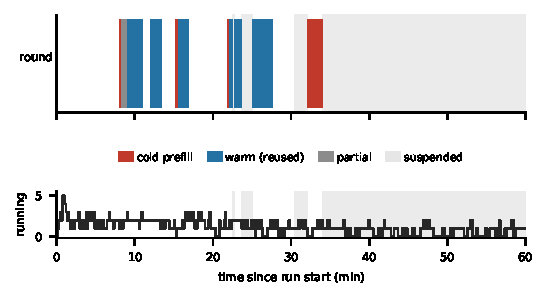
\includegraphics[width=\columnwidth]{figs/fig_timeline.pdf}
\caption{One session of the capacity-accounted arm (39 rounds, 17 suspensions), first hour.
Each bar is a round, coloured by how much of its prefix the engine had to recompute; grey
spans are suspensions. The lower panel is the engine's running-request count: while the
session is suspended the card keeps serving other sessions, which is the slot the
suspension buys. A round that follows a suspension is usually red---the state did not
survive---which is the cost side of the same decision.}
\label{fig:timeline}
\end{figure}

\pend{paragraph reading the timeline: how often the session was suspended, what the
suspension cost (revival vs recompute counts), and whether the slot was picked up by
another session while it was parked.}

\subsection{Log-based counterfactual: concurrency or state?}
\label{sec:eval-cf}

Our design differs from the agent-level baseline in two ways at once: it accounts for
capacity, and it preserves state. To separate the two without another run, we replay the
controller's own decisions offline and ask what would have happened under a concurrency-only
variant of the same controller---same permits, same pausing, but no host-tier accounting
and no revival pricing.

\pend{the counterfactual numbers and the sentence that says how much of the gain comes from
each half.}

\subsection{When it does not pay}
\label{sec:eval-neg}

We report three regimes in which the mechanism loses or is neutral, and we say why.
\emph{(i) Ample capacity.} If the working set fits, nothing is suspended, the ledger reduces
to first-come-first-served, and the only difference from the request-level arm is a small
amount of bookkeeping; the design cannot win and does not claim to. \emph{(ii) Short
contexts.} If a round's context is small, the recompute is cheap and the break-even
\eqref{eq:ratio} favours recomputation; suspension then buys nothing. \emph{(iii) Saturated
engine.} When the engine is already busy, adding admission discipline removes capacity from
the queue and can increase the tail, because the door wait moves from a place where it
overlaps with other work to a place where it does not.

\pend{the measured instances of (i)--(iii) in the arms, and the sensitivity to $\rho$ and
$t^\ast$.}

\subsection{Threats to validity}
\label{sec:eval-threats}

Every arm is a single run of one trace on one GPU, so we report measured differences and
full distributions rather than significance tests; run-to-run variation is visible only in
the per-session scatter, and a single batch cannot separate policy effects from the
particular interleaving. The trace is reconstructed from agent transcripts rather than
observed in production, and all sessions arrive together, which is the worst case for
admission and the best case for a batch controller. The model is a 7B coding model on a
24\,GB card; the constants in \S\ref{sec:analysis} would differ on other hardware, though
the quantities in which the argument is stated would not.

\section{Related Work}
\label{sec:related}

\paragraph{KV memory in serving engines.} PagedAttention \cite{kwon2023pagedattention}
made the KV cache a paged allocator, and SGLang \cite{zheng2024sglang} made prefix sharing a
first-class citizen through a radix tree; both are the substrate we stand on and neither has
a notion of a session. Hierarchical and disaggregated stores extend the hierarchy---host
memory, remote tiers, and prefill/decode separation \cite{mooncake,distserve}---and answer
\emph{where} a block should live. Our question is prior to theirs: given that the hierarchy
exists, which session is allowed to occupy the fast tier, and what does it cost to bring one
back. Pensieve \cite{yu2025pensieve} argued that statelessness is the structural fault of
current serving designs; we make the same argument quantitatively and add the admission
decision that statelessness leaves open.

\paragraph{Scheduling for agentic and multi-turn workloads.} CONCUR \cite{concur} controls
concurrency at agent granularity with an AIMD law driven by a congestion signal, and it is
the closest system to ours in scope; our agent-level arm is deliberately a faithful
reimplementation of that control law, so that the comparison isolates the decision rule. We
differ in what is being decided: AIMD adjusts a window and reacts after congestion appears,
whereas the ledger tests feasibility before admitting and prices what happens when it
cannot. Continuum \cite{continuum} attaches a time-to-live to a session's KV and uses cache
miss cost to schedule, which is a prediction of the reuse window; our reserve is a
measurement of growth, not of a horizon. KVFlow \cite{kvflow} predicts
steps-to-execution to schedule workflows, and ThunderAgent \cite{thunderagent} decomposes
program cost in space and time; both model the future of a program, and both would benefit
from a feasibility layer underneath. Talaria \cite{talaria} targets session continuity in
serverless serving, and ConServe changes the scheduling unit;
% TODO(cite): ConServe arXiv:2606.01839 — 标题/作者核过后加进 refs.bib we change
what the unit is allowed to own. MORI \cite{mori} exploits tool-call idle windows to offload
per tier, and EfficientAgent admits by working set
% TODO(cite): EfficientAgent arXiv:2609.33762 — 标题/作者核过后加进 refs.bib and ranks sessions
for eviction by expected reuse; our problem statement overlaps theirs, and we make no claim
of novelty on granularity, tiers, or working-set admission as such. The claim here is that
the decision can be stated as a feasibility test with a measured ledger and a priced
recovery, without a predictor of future demand.

\paragraph{Measurement of agentic workloads.} A recent characterisation of production
agentic traffic reports
% TODO(cite): KV Residency arXiv:2610.22863 — 标题/作者核过后加进 refs.bib session lifetimes and per-session KV footprints
at a scale where the aggregate working set would need hundreds of terabytes to hold; the
conclusion there is that hold-all-live is impossible, which is the regime we make precise on
one card: a working set $12.9\times$ the pool, a pool that holds 1.47 mean sessions, and a
13$\times$ re-read tax paid by request-level serving. Our trace is a replay built from
coding-agent transcripts \cite{zhu2026tracelab}, so it inherits their structure rather than
observing a deployment; we state that as a threat to validity rather than as evidence of
production behaviour.

\paragraph{Admission and overload control.} Classical admission control reacts to
utilisation with multiplicative decrease \cite{jacobson1988}; the working-set model
\cite{denning1978} and Little's law \cite{little1961} describe when a set of jobs fits in
memory and what concurrency a throughput target implies. We use the same vocabulary but a
different object: the working set here is a set of \emph{sessions} with reusable state, so
the cost of admitting the wrong one is not queueing delay but recomputation, and the
relevant invariant is a byte budget rather than a window. Overload handlers that reject
requests \cite{mooncake} are the limiting case of our design in which every suspension is
made permanent; our point is that a rejection can be made reversible, and that the
break-even (\S\ref{sec:analysis}) says when it should not be.

\section{Discussion}
\label{sec:discussion}

\paragraph{What the argument is, and is not} The claim is not that this card, this model,
or this trace is representative. It is that once sessions can be suspended, admission stops
being a forecast and becomes a feasibility test with a price, and that this reframing is
what turns an unmanaged pool into a usable server under working-set overcommitment. The
quantities in which the argument is stated---bytes of KV, bytes per second between tiers,
rounds per session, rounds per second of prefill---are measurable on any deployment; the
constants are not portable, and we do not present them as such.

\begin{table}[t]
\caption{The regime the design targets, and where it does not apply.}
\label{tab:scope}
\centering
\small
\begin{tabular}{@{}p{0.44\columnwidth}p{0.46\columnwidth}@{}}
\toprule
Applies & Does not apply \\
\midrule
working set $\gg$ KV pool: long sessions, large contexts &
working set well below the pool: nothing is suspended and the ledger is inert \\
single node with a host tier that can hold suspended state &
cluster-level disaggregation, where placement is a different problem \\
contexts large enough that recomputation dominates a copy &
contexts short enough that the recompute is cheaper than the revival \\
sessions that return: multi-round jobs with reusable prefixes &
one-shot requests, where there is no state to preserve \\
\bottomrule
\end{tabular}
\end{table}

\paragraph{Why the negative cases matter} A design of this kind is easy to oversell,
because every mechanism in it can be made to look good on the workload it was tuned for.
The three losing regimes in \S\ref{sec:eval-neg} are therefore part of the result: they
delineate the ratio of working set to capacity at which accounting stops being the
interesting question, and they explain why threshold controllers are not simply mistakes---
in a regime where the working set is small, a window is a perfectly good answer, and the
ledger has nothing to add.

\paragraph{Implications for systems that already have a hierarchy} The mechanism does not
require a new engine. It requires that the engine expose enough for a controller to keep
books---token usage, running counts, per-request cache accounting---and that the scheduler
allow a request to be held at a session boundary rather than only admitted or dropped.
Both are interface changes, not algorithmic ones, and both are absent from current engines
mainly because the request, not the session, is their unit of work.

\paragraph{Threats beyond the evaluation} Our replay arrives all at once, which makes
admission hardest and makes a batch controller look good; a Poisson arrival process would
give the request-level arm more slack and shrink the measured gap, though it would not
change which decisions are feasible. The trace's tool waits are simulated from the
recorded distribution rather than observed live, so the interaction between admission
delays and agent behaviour (an agent that waits longer may emit a longer next round) is
not modelled. Both are directions for measurement rather than for mechanism.

\section{Conclusion}
\label{sec:conclusion}

Serving agents is not serving requests. A session arrives with state, leaves it behind, and
comes back to it, and on a single GPU the aggregate of that state exceeds the pool by an
order of magnitude. The systems we have are built around a threshold---how many, how much
concurrency, how high a watermark---which forces the operator to guess at a future the
workload does not reveal until it happens.

Once a session can be suspended and revived, the guess is unnecessary. Capacity becomes a
ledger of bytes, admission becomes a feasibility test against that ledger, and the two
decisions that remain---whose state deserves a slot, and whether to copy or recompute---are
priced in measured time. The design needs no predictor of the next round, and the numbers
say why: the part of the footprint that would have to be predicted is a few percent of the
part that is measured.

We have instantiated the principle as a controller outside an unmodified serving engine and
measured it against request-level serving and an agent-level feedback controller on a
19-session coding-agent replay. \pend{one-sentence result with the three arms}. The
reusable part is not the constants but the shape of the argument: state the feasible set,
price the recovery, and let the workload decide---rather than tune a threshold and hope the
next round looks like the last.


\bibliographystyle{IEEEtran}
\bibliography{refs}

\end{document}
